%
% Projekt do předmětu Grafové algoritmy -- GAL (Generování bludišť)
% Autor: Vojtěch Havlena <xhavle03@stud.fit.vutbr.cz>
% Datum: 10. 11. 2015
%

\documentclass[a4paper,12pt]{article}

\usepackage[utf8]{inputenc}
\usepackage[czech]{babel}
\usepackage[IL2]{fontenc}
\usepackage[left=3cm,text={15cm, 23cm},top=3.5cm]{geometry}
\usepackage{subcaption}

\usepackage{color}
\usepackage[ruled,czech,linesnumbered,noline]{algorithm2e}
\usepackage{graphicx}

\usepackage{tikz}
\usetikzlibrary{patterns}

\definecolor{grey}{rgb}{0.745098,0.745098,0.745098}

\usepackage{amssymb}
\usepackage{amsmath}
\usepackage{amsthm}

\begin{document}

%
% Projekt do předmětu Grafové algoritmy -- GAL (Generování bludišť)
% Autor: Vojtěch Havlena <xhavle03@stud.fit.vutbr.cz>
% Datum: 10. 11. 2015
%

\begin{titlepage}

\vfill~

\begin{center}
  \bigskip
  {\Huge Generování bludišť\\}
  {\Large Projekt rešerše do předmětu GAL\\}
\end{center}

\vfill

\begin{center}
  {\Large \today }
\end{center}

\vfill

\begin{flushleft}
  {\large 
  \begin{tabular}{ll}
    Autor: & Vojtěch Havlena (xhavle03) \\
    & Fakulta Informačních Technologií \\
    & Vysoké Učení Technické v~Brně \\
    \end{tabular} }
\end{flushleft}
\end{titlepage}


\tableofcontents
\newpage

\section{Úvod}
Pod pojmem bludiště lze chápat systém spletitých cest a slepých uliček \cite{wiki}. Řešením bludiště
je potom nalezení cesty z~počátečního do koncového bodu. Často se pojem bludiště nahrazuje pojmem
labyrint, nicméně labyrint ve většině případů označuje jednu klikatou cestu z~počátečního 
do koncového bodu \cite{ped}. Labyrintům se v~této práci dále věnovat nebudeme. Tato práce se zabývá 
algoritmy pro generování bludišť, zejména se jedná o~algoritmy založené na teorii grafů.

Pravděpodobně primárním využitím bludišť je pobavení lidí. Řešení bludišť může být určeno pro 
lidi různých věkových kategorií. S~rovinnými bludišti se můžeme setkat například v~různých 
časopisech pro pobavení čtenářů. Bludiště se také často využívají v~počítačových hrách, kde
náhodně vytvořené prostředí, ve kterém se hráč pohybuje, lze považovat za určitý typ bludiště.
Bludiště se také dají využít pro testování inteligence a orientačních schopností různých živočichů.

\subsection{Prvky bludiště a typy bludišť}
Základními stavebními prvky bludišť jsou zeď a buňka. Buňkou rozumíme základní element
v~bludišti. Zdi od sebe oddělují sousední buňky, mezi kterými neexistuje přímé propojení.
Podle počtu propojení se sousedními buňkami dělíme buňky na: izolované (0 propojení), slepý konec (1 propojení)
buňka součástí cesty (2 propojení) a křižovatka (3 a více propojení). Cestou v~bludišti pak rozumíme souvislou
posloupnost propojených buněk.

Bludiště se mohou rozdělovat podle několika hledisek. Prvním takovým dělením je dělení podle typu dimenze. 
Základními typy jsou dvoudimenzionální a třídimenzionální bludiště \cite{pul:lab}.
U~více dimenzionálních bludišť nastává problém s~vizualizací takového bludiště. Proto se často 
více dimenzionální bludiště zobrazují jako dvou, popř. třídimenzionální bludiště spojená portály\footnote{Lze si 
představit jako teleporty, které přenášejí procházející objekt mezi bludišti.}.
V~této práci se však budeme zabývat zejména dvoudimenzionálními bludišti. 

Dále je možné uvažovat dělení podle vnitřní struktury. Zde rozlišujeme tzv. perfektní bludiště, pro které platí, že
mezi libovolnými dvěma body vede vždy jen jedna cesta. Pokud bludiště obsahuje cykly, ale neobsahuje slepé konce, jedná
se o~spletené bludiště. V~případě, že spletené bludiště obsahuje slepé konce, hovoříme o~něm jako o~částečně spleteném bludišti.
Nakonec, pokud bludiště obsahuje oddělené části, nazývá se řídké \cite{pul:lab}.

Posledním zmíněným dělením, které zohledňuje především vzhled bludiště, je dělení podle typu mozaiky \cite{pul:lab}.
Toto dělení se zaměřuje na vzhled buněk. Základním a jediným typem, který je v~práci uvažován, jsou
ortogonální bludiště, tedy bludiště se čtvercovými buňkami. Dále je možné uvažovat trojúhelníkové buňky (delta bludiště),
šestiúhelníkové buňky (sigma bludiště) a jiné.

V~další části práce se již budeme věnovat samotným algoritmům pro generování různých typů bludišť.
Také se budeme zabývat souvislostí mezi generováním bludišť a teorií grafů.

\section{Generování založené na teorii grafů}
V~této kapitole se budeme zabývat generováním bludišť s~využitím teorie grafů.
V~případě, že budeme uvažovat ortogonální (pravoúhlá) bludiště, je možné reprezentovat strukturu bludiště pomocí rovinného
neorientovaného grafu (mřížky) \cite{mat}. Každý uzel grafu reprezentuje jednu buňku bludiště. Hrany grafu potom představují přechody
mezi sousedními buňkami v~bludišti. Příklad této reprezentace je na obr.~\ref{fig:mazeReprezentation}. Hlavní výhodou 
této reprezentace je abstrakce od grafického zobrazení bludiště (velikost, tvar buněk apod.). 

\begin{figure}[h]
  \begin{center}
  \begin{tikzpicture}
  \foreach \x in {0,...,3}
    \foreach \y in {0,...,3}
    {
      \fill (\x,\y) circle (2pt);
    }
  
  \draw [step=1.0,black] (0,0) grid (3,3);
  
  \foreach \x in {0,...,3}
    \foreach \y in {0,...,3}
    {
      \fill (\x + 5,\y) circle (2pt);
    }
   
   \draw [->,thick] (3.5, 1.5) -- (4.5,1.5);
   
   \draw (5,3) -- (6,3);
   \draw (6,3) -- (6,2);
   \draw (6,2) -- (7,2);
   \draw (7,2) -- (7,0);
   \draw (7,1) -- (8,1);
   \draw (8,1) -- (8,0);
   \draw (7,2) -- (8,2);
   \draw (8,3) -- (8,2);
   \draw (6,3) -- (7,3);
   \draw (5,3) -- (5,0);
   \draw (5,1) -- (6,1);
   \draw (6,1) -- (6,0);
   
   \draw node at (9,1.5) {\LARGE $\approx$};
   
   \draw (10, -0.5) rectangle (14,3.5);
   \draw (11,-0.5) -- (11,0.5);
   \draw (11,1.5) -- (11,2.5);
   \draw (11,1.5) -- (12,1.5);
   \draw (12,1.5) -- (12,-0.5);
   \draw (12,2.5) -- (13,2.5);
   \draw (13,2.5) -- (13,3.5);
   \draw (13,1.5) -- (14,1.5);
   \draw (13,-0.5) -- (13,0.5);
  \end{tikzpicture}
  \end{center}
  \caption{Neorientovaný graf reprezentující bludiště o~rozměru 4$\times$4 bez zdí. Vynecháním některých hran vznikne 
  graf odpovídající bludišti na posledním obrázku.}
  \label{fig:mazeReprezentation}
\end{figure}

Pro generování bludišť založené na teorii grafů se vychází z~generování perfektního bludiště. Pro zopakování, perfektní bludiště je 
bludiště, ve kterém mezi libovolnými dvěma buňkami existuje právě jedna cesta. Tato definice odpovídá definici stromu v~teorii grafů.
Využijeme-li reprezentaci bludiště popsanou výše, generování perfektního bludiště odpovídá hledání kostry grafu. V~další části se 
tedy budeme věnovat modifikacím algoritmů pro hledání kostry grafu tak, aby byly schopny generovat perfektní bludiště.

\subsection{Randomizovaný Primův algoritmus}
První představený algoritmus použitelný pro generování perfektního bludiště je randomizovaný Primův algoritmus \cite{fol}. Jak již ale bylo zmíněno dříve,
bludiště reprezentujeme pomocí neorientovaného neohodnoceného grafu. Proto si graf reprezentující bludiště můžeme představit tak, že každé hraně je přiřazena 
konstantní váha $1$ a Primův algoritmus tedy může hrany do minimální kostry vybírat náhodně.

Varianta tohoto algoritmu používaná pro generování bludišť využívá rozdělování buněk (uzlů) do tří množin -- uvnitř ($U$), pomezí ($P$) a mimo ($M$).
Množina $U$ obsahuje buňky, které již jsou součástí bludiště. Množina $M$ obsahuje buňky, které ještě nejsou součástí bludiště a 
nakonec množina $P$ obsahuje buňky, které ještě nejsou součástí bludiště, ale mají alespoň jednoho souseda v~množině $U$.

Na začátku algoritmu se po inicializaci vybere počáteční buňka a ta se přesune do množiny $U$. Všichni její sousedé se přesunou do množiny $P$.
Následně se opakovaně vybírají buňky z~množiny $P$, dokud tato množina není prázdná. Každá vybraná buňka se přesune do množiny $U$, 
poznačí se možnost přechodu v~bludišti mezi vybranou buňkou a sousední buňkou, která je již v~množině $U$ (přidá se hrana mezi odpovídajícími 
uzly do grafu bludiště). Následně se aktualizuje obsah množin $P$ a $M$ \cite{mat,fol}. Příklad generování bludiště je na obr.~\ref{fig:prim}. 
Zápis v~pseudokódu je následující:

\medskip

 \begin{algorithm}[H]
 \SetKwInput{Input}{Vstup}\SetKwInOut{Output}{Výstup}
 \SetNlSty{}{}{:}
 \SetNlSkip{-1.0em}
 \SetInd{0.5em}{0.5em}
 \Input{Graf $G = (V, E)$ reprezentující bludiště bez vnitřních zdí.}
 \Output{Perfektní bludiště}
 \BlankLine
 \Indentp{1.7em}
   Do množiny $M$ ulož všechny buňky bludiště ($M\gets V$), $P \gets \emptyset$, $U \gets \emptyset$. \\
   Náhodně vyber počáteční buňku bludiště $s$ a přidej ji do množiny $U$.\\
   Přidej do množiny $P$ všechny sousední buňky buňky $s$. \\
   \While{$P \neq \emptyset$}
   {
     Vyber náhodně buňku $c_P$ z~množiny $P$ \\
     Vyber náhodně buňku $c_U \in U$ takovou, že $c_U$ je sousední buňka $c_P$. \\
     $U \gets U \cup \{ c_P \}$ \\
     Přesuň všechny sousední buňky $c_P$, které jsou v~množině $M$ z~množiny $M$ do $P$. \\
     Poznač spojení v~bludišti mezi buňkami $c_P$ a $c_U$. \\
     $P \gets P \setminus \{ c_P \} $.
     }
 \caption{\textsc{Modifikovaný randomizovaný Primův algoritmus}}
 \label{alg:prim}
\end{algorithm}

\medskip
Tento algoritmus lze upravit tak, aby generoval i bludiště obsahující cykly (tedy ne již perfektní bludiště). 
Modifikace spočívá v~tom, že se náhodně vybraná buňka $c_P$ z~množiny $P$ s~určitou pravděpodobností 
z~množiny $P$ neodebere (úprava řádku~10). Opětovným výběrem této buňky potom vznikne v~bludišti cyklus \cite{mat}.

\begin{figure}[h]
  \begin{center}
  \begin{tikzpicture}[scale=0.7]  

   \draw[fill=gray!20!white, draw=black] (0,0) grid (4,4) rectangle (0,0);
   \filldraw[fill=white, draw=black] (1,2) rectangle (2,3);
   \draw[pattern=north west lines, pattern color=black] (0,2) rectangle (1,3);
   \draw[pattern=north west lines, pattern color=black] (1,3) rectangle (2,4);
   \draw[pattern=north west lines, pattern color=black] (1,1) rectangle (2,2);
   \draw[pattern=north west lines, pattern color=black] (2,2) rectangle (3,3);

   \draw [->,thick] (4.2, 2) -- (5.2,2);
   
  \end{tikzpicture}
  \begin{tikzpicture}[scale=0.7]  

   \draw[fill=gray!20!white, draw=black] (0,0) grid (4,4) rectangle (0,0);
   \filldraw[fill=white, draw=black] (1,2) rectangle (3,3);
   \draw[pattern=north west lines, pattern color=black] (0,2) rectangle (1,3);
   \draw[pattern=north west lines, pattern color=black] (1,3) rectangle (2,4);
   \draw[pattern=north west lines, pattern color=black] (1,1) rectangle (2,2);
   \draw[pattern=north west lines, pattern color=black] (3,2) rectangle (4,3);
   \draw[pattern=north west lines, pattern color=black] (2,1) rectangle (3,2);
   \draw[pattern=north west lines, pattern color=black] (2,3) rectangle (3,4);

   \draw [->,thick,dashed] (4.2, 2) -- (5.2,2);
  \end{tikzpicture}
  \begin{tikzpicture}[scale=0.7]  

   \draw[fill=gray!20!white, draw=black] (0,0) grid (4,4) rectangle (0,0);
   \fill[fill=white] (1,2) rectangle (3,3);
   \fill[fill=white] (2,3) rectangle (3,0);
   \fill[fill=white] (2,1) rectangle (4,2);
   \draw (0,0) rectangle (4,4);
   
   \draw[pattern=north west lines, pattern color=black] (0,2) rectangle (1,3);
   \draw[pattern=north west lines, pattern color=black] (1,3) rectangle (2,4);
   \draw[pattern=north west lines, pattern color=black] (1,1) rectangle (2,2);
   \draw[pattern=north west lines, pattern color=black] (3,2) rectangle (4,3);
   \draw[pattern=north west lines, pattern color=black] (2,3) rectangle (3,4);
   \draw[pattern=north west lines, pattern color=black] (1,0) rectangle (2,1);
   \draw[pattern=north west lines, pattern color=black] (3,0) rectangle (4,1);

   \draw [->,thick,dashed] (4.2, 2) -- (5.2,2);
  \end{tikzpicture}
  \begin{tikzpicture}[scale=0.7]  
   \draw (10, -0.5) rectangle (14,3.5);
   \draw (11,-0.5) -- (11,0.5);
   \draw (11,1.5) -- (11,2.5);
   \draw (11,1.5) -- (12,1.5);
   \draw (12,1.5) -- (12,-0.5);
   \draw (12,2.5) -- (13,2.5);
   \draw (13,2.5) -- (13,3.5);
   \draw (13,1.5) -- (14,1.5);
   \draw (13,-0.5) -- (13,0.5);
  \end{tikzpicture}
  \end{center}
  \caption{Příklad generování bludiště randomizovaným Primovým algoritmem. Bílou barvou jsou označeny buňky v~množině $U$, plnou šedou barvou buňky v~množině $M$ a
  čárkovaně buňky v~$P$.}
  \label{fig:prim}
\end{figure}
 
\subsection{Randomizovaný Kruskalův algoritmus}
Další algoritmus, použitelný pro generování perfektního bludiště, je randomizovaný Kruskalův algoritmus \cite{fol}. Vzhledem k~tomu, že 
graf reprezentující bludiště je neohodnocený neorientovaný graf, rozšíříme si tento graf o~konstantní ohodnocení $1$ každé hraně (podobně jako
v~případě randomizovaného Primova algoritmu). Jediná modifikace oproti původnímu Kruskalově algoritmu je, že hrany se z~množiny dosud nepoužitých hran
vybírají náhodně.

V~prvním kroku algoritmu se provede vytvoření množin pro každou buňku (resp. uzel v~grafu). V~dalším kroku se opakovaně náhodně vybírá zeď (resp. hrana v~grafu) 
z~množiny zdí, dokud množina zdí není prázdná. Pokud jsou obě buňky, které jsou touto zdí odděleny, v~různých množinách, obě tyto množiny se sjednotí a 
poznačí se cesta mezi těmito buňkami. V~případě, že buňky jsou ve stejných množinách, není možné zeď odstranit. Vybraná zeď je posléze odstraněna z~množiny zdí.
Příklad generování bludiště je na obr.~\ref{fig:kruskal}.

\begin{figure}[h]
  \begin{center}
  \begin{tikzpicture}[scale=0.7]  

   \draw[fill=white, draw=black] (0,0) grid (4,4) rectangle (0,0);
   \draw node at (2.5, 1) {$\times$};
   
   \draw [->,thick] (4.2, 2) -- (5.2,2);
   
  \end{tikzpicture}
  \begin{tikzpicture}[scale=0.7]  
   \draw[fill=white, draw=black] (0,0) grid (4,4) rectangle (0,0);
   \draw node at (1.5, 1) {$\times$};
   
   \filldraw[fill=white] (2,0) rectangle (3,2);
   
   \draw [->,thick,dashed] (4.2, 2) -- (5.2,2);
  \end{tikzpicture}
  \begin{tikzpicture}[scale=0.7]  
  \draw[fill=white, draw=black] (0,0) grid (4,4) rectangle (0,0);
   
   
   \filldraw[fill=white] (2,0) rectangle (4,2);
   \filldraw[fill=white] (1,0) rectangle (2,2);
   \filldraw[fill=white] (0,0) rectangle (1,4);
   \filldraw[fill=white] (2,2) rectangle (4,3);
   \draw (3,0) -- (3,1);
   
   \draw node at (1, 1.5) {$\times$};

   \draw [->,thick,dashed] (4.2, 2) -- (5.2,2);
  \end{tikzpicture}
  \begin{tikzpicture}[scale=0.7]  
   \draw (10, -0.5) rectangle (14,3.5);
   \draw (11,-0.5) -- (11,0.5);
   \draw (11,1.5) -- (11,2.5);
   \draw (11,1.5) -- (12,1.5);
   \draw (12,1.5) -- (12,-0.5);
   \draw (12,2.5) -- (13,2.5);
   \draw (13,2.5) -- (13,3.5);
   \draw (13,1.5) -- (14,1.5);
   \draw (13,-0.5) -- (13,0.5);
  \end{tikzpicture}
  \end{center}
  \caption{Příklad generování bludiště randomizovaným Kruskalovým algoritmem.}
  \label{fig:kruskal}
\end{figure}
Podobně jako v~případě randomizovaného Primova algoritmu, i tento algoritmus lze modifikovat pro generování 
bludišť obsahující cykly. Modifikace spočívá v~tom, že pokud nějakou zeď nemůžeme odebrat, tak ji s~určitou
pravděpodobností přesto odebereme. Tím pádem nám vzniknou cykly \cite{mat}.
 
\subsection{Prohledávání do hloubky}
Dalším algoritmem, který lze použít pro generování kostry grafu a tedy i perfektního bludiště, je 
prohledávání do hloubky (DFS) \cite{mat, fol}. Vstupem algoritmu DFS je graf reprezentující bludiště bez vnitřních stěn. Vzhledem k~tomu, že zmíněný graf je souvislým grafem,
je i les prohledávání do hloubky souvislým grafem a tedy stromem.

Jediný rozdíl oproti klasickému algoritmu DFS je způsob volby buněk (uzlů) pro další procházení. Aby bludiště vypadalo co
nejvíce nepravidelně, je počáteční buňka zvolena náhodně. Stejně tak sousední buňky jsou v~proceduře \textsc{Dfs-visit}~\cite{gal} vybírány v~náhodném pořadí.
Nevýhodou tohoto algoritmu je použití rekurze, což zejména pro generování velkých bludišť způsobuje problémy. Proto se pro generování
častěji využívá modifikace DFS nepoužívající rekurzi, ale využívající vlastní zásobník.
Příklad generování bludiště je uveden na obr.~\ref{fig:dfs}. 

\begin{figure}[h]
  \begin{center}
  \begin{tikzpicture}[scale=0.7]  

   \draw[fill=white, draw=black] (0,0) grid (4,4) rectangle (0,0);
   \filldraw[fill=gray!20!white, draw=black] (1,0) rectangle (2,1);
   
   \draw [->,thick,dashed] (4.2, 2) -- (5.2,2);
   
  \end{tikzpicture}
  \begin{tikzpicture}[scale=0.7]  
   \draw[fill=white, draw=black] (0,0) grid (4,4) rectangle (0,0);
   
   \filldraw[fill=white] (0,0) rectangle (2,2);
   \draw (1,0) -- (1,1);
   \draw (1.5, 0.5) -- (1.5, 1.5) -- (0.5, 1.5);
   \draw[->] (0.5, 1.5) -- (0.5, 0.5);
   
   \draw [->,thick,dashed] (4.2, 2) -- (5.2,2);
  \end{tikzpicture}
  \begin{tikzpicture}[scale=0.7]  
    \draw[fill=white, draw=black] (0,0) grid (4,4) rectangle (0,0);
   
   \filldraw[fill=white] (0,0) rectangle (4,3);
   \draw (1,0) -- (1,1);
   \draw (2,0) -- (2,2);
   \draw (1,2) -- (3,2);
   \draw (3,1) -- (4,1);
   
   \draw (0.5, 1.5) -- (0.5, 2.5) -- (3.5, 2.5) -- (3.5, 1.5) -- (2.5, 1.5) -- (2.5, 0.5);
   \draw[->] (2.5, 0.5) -- (3.5, 0.5);
   
   \draw [->,thick,dashed] (4.2, 2) -- (5.2,2);
  \end{tikzpicture}
  \begin{tikzpicture}[scale=0.7]  
   \filldraw[fill=white] (0,0) rectangle (4,4);
   \draw (1,0) -- (1,1);
   \draw (2,0) -- (2,2);
   \draw (1,2) -- (3,2);
   \draw (3,1) -- (4,1);
   \draw (0,3) -- (3,3);
  \end{tikzpicture}
  \end{center}
  \caption{Příklad generování bludiště algoritmem DFS. Šedou barvou je označena počáteční buňka.}
  \label{fig:dfs}
\end{figure}

Výhodou tohoto algoritmu je lineární časová složitost (vzhledem k~reprezentaci grafu bludiště).
Nevýhodou je fakt, že ne všechny perfektní bludiště je algoritmem DFS možné vygenerovat. Například bludiště na obr.~\ref{fig:mazeReprezentation}
není možné tímto algoritmem vygenerovat.

\subsection{Aldous--Broderův algoritmus}
Další algoritmus, který lze použít pro generování perfektního bludiště, úzce souvisí s~pojmem rovnoměrná kostra grafu (uniform spanning tree).
Rovnoměrná kostra grafu je kostra grafu, která byla náhodně (a se stejnou pravděpodobností) vybrána ze všech možných koster daného grafu \cite{mat}.
Pro hledání rovnoměrných koster lze využít právě Aldous--Broderův algoritmus. Rovnoměrné kostry mají využití např. v~kombinatorice nebo
ve fyzice (konkrétně v~oblasti kvantové teorie pole) \cite{span}.

Vstupem algoritmu je neorientovaný souvislý graf. Výstupem je rovnoměrná kostra zadaného grafu. Principem algoritmu je náhodné procházení 
grafu. Na začátku algoritmu se náhodně zvolí libovolný uzel grafu $u$ a tento uzel označ jako 
navštívený. V~dalším kroku náhodně vyber jeden
sousední uzel $v$ uzlu $u$, který je s~uzlem $u$ spojen hranou. Pokud uzel $v$ ještě nebyl navštíven, přidej hranu $(u, v)$ do 
kostry grafu. Nakonec se přesuň do uzlu $v$, tedy $u\gets v$. Následně pokračuj na krok výběru jednoho sousedního uzlu a tento
výběr opakuj dokud nejsou všechny uzly grafu označeny jako navštívené \cite{ald, mat}.

Popsaný algoritmus lze snadno modifikovat pro generování bludiště \cite{mat}. Vstupem algoritmu bude graf reprezentující bludiště bez vnitřních zdí.
Algoritmus pro generování popsaný v~pseudokódu je potom následující.

\medskip

 \begin{algorithm}[H]
 \SetKwInput{Input}{Vstup}\SetKwInOut{Output}{Výstup}
 \SetNlSty{}{}{:}
 \SetNlSkip{-1.0em}
 \SetInd{0.5em}{0.5em}
 \Input{Graf $G = (V, E)$ reprezentující bludiště bez vnitřních zdí.}
 \Output{Perfektní bludiště.}
 \BlankLine
 \Indentp{1.7em}
   Náhodně vyber buňku bludiště $u$. \\
   Inicializuj množinu navštívených buněk $Vis \gets \emptyset$.\\
   \Repeat{$|Vis| = |V|$}
   {
     $Vis \gets Vis \cup \{ u \}$ \\
     Náhodně vyber sousední buňku $u'$ buňky $u$.\\
     \If{$u' \not\in Vis$}
     {
	Poznač spojení mezi buňkami $u$ a $u'$.\
     }
     $u \gets u'$
     }
 \caption{\textsc{Aldous--Broderův algoritmus}}
 \label{alg:aldous}
\end{algorithm}

\medskip

Výhodou Aldous--Broderova algoritmu je jeho jednoduchost a možnost generovat libovolné perfektní bludiště. Nevýhodou je jeho značná neefektivnost.

\enlargethispage*{0.5em}
Kromě Aldous--Broderova algoritmu lze pro hledání rovnoměrných koster grafu využít také Wilsonův algoritmus. Wilsonův algoritmus 
provede v~daném grafu náhodnou procházku a odstraní cykly vzniklé při této procházce. Na rozdíl od Aldous--Broderova algoritmu
má ale Wilsonův algoritmus zaručenou polynomiální časovou složitost \cite{span}.

\subsection{Algoritmus Hunt and Kill}
Poslední představený algoritmus, založený na teorii grafů, který lze použít pro generování perfektního bludiště, je algoritmus
Hunt and Kill \cite{fol}. Algoritmus Hunt and Kill se dá považovat za jistou modifikaci prohledávání do hloubky.

Algoritmus provádí průchod grafem s~náhodným výběrem nenavštíveného sousedního uzlu, do kterého se bude pokračovat. V~případě, že
žádný nenavštívený sousední uzel neexistuje, na rozdíl od prohledávání do hloubky (backtrackingu), kde se provede návrat k~předcházejícímu uzlu,
v~případě algoritmu Hund and Kill se provede návrat do libovolného již navštíveného uzlu, který obsahuje alespoň jednoho nenavštíveného souseda.
Z~tohoto uzlu se potom pokračuje v~průchodu grafu.

Algoritmus v~pseudokódu přizpůsobený pro generování bludišť je potom zapsán následovně.

\medskip

 \begin{algorithm}[H]
 \SetKwInput{Input}{Vstup}\SetKwInOut{Output}{Výstup}
 \SetNlSty{}{}{:}
 \SetNlSkip{-1.0em}
 \SetInd{0.5em}{0.5em}
 \Input{Graf $G = (V, E)$ reprezentující bludiště bez vnitřních zdí.}
 \Output{Perfektní bludiště.}
 \BlankLine
 \Indentp{1.7em}
   Náhodně vyber buňku bludiště $u$. \\
   Inicializuj množinu navštívených buněk $Vis \gets \{u\}$.\\
   \While{$|Vis| \neq |V|$}
   {
     \uIf{$u$ má nenavštívené sousední buňky}
     {
	Náhodně vyber buňku $v$ z~množiny nenavštívených sousedních buněk~$u$.\\
	Poznač spojení mezi buňkami $u$ a $v$. \\
	$u\gets v$ \\
	$Vis \gets Vis \cup \{u\}$
     }
     \Else
     {
        Náhodně vyber buňku $u$ z~množiny již navštívených buněk, které mají alespoň jednu nenavštívenou sousední buňku.
     }
     }
 \caption{\textsc{Algoritmus Hunt and Kill}}
 \label{alg:huntkill}
\end{algorithm}

\medskip
\enlargethispage{1em}
Výhodou tohoto algoritmu oproti algoritmu DFS je možnost generovat bludiště, které pomocí DFS vygenerovat nelze. 
Např. bludiště na obr.~\ref{fig:hk} není možné algoritmem DFS vygenerovat. Nicméně na druhou stranu existují i perfektní bludiště,
které není možné algoritmem Hunt and Kill vygenerovat.

\begin{figure}[h]
  \begin{center}
  \begin{tikzpicture}[scale=0.7]  

   \draw[fill=white, draw=black] (0,0) grid (4,4) rectangle (0,0);
   \filldraw[fill=gray!20!white, draw=black] (1,0) rectangle (2,1);
   
   \draw [->,thick,dashed] (4.2, 2) -- (5.2,2);
   
  \end{tikzpicture}
  \begin{tikzpicture}[scale=0.7]  
   \draw[fill=white, draw=black] (0,0) grid (4,4) rectangle (0,0);
   
   \filldraw[fill=white] (1,0) rectangle (4,2);
   \draw (2,0) -- (2,1) -- (3,1);
   
   
   \draw (1.5, 0.5) -- (1.5, 1.5) -- (3.5, 1.5) -- (3.5, 0.5);
   \draw[->] (3.5, 0.5) -- (2.5, 0.5);
   
   \draw [->,thick,dashed] (4.2, 2) -- (5.2,2);
  \end{tikzpicture}
  \begin{tikzpicture}[scale=0.7]  
    \draw[fill=white, draw=black] (0,0) grid (4,4) rectangle (0,0);
    \filldraw[fill=gray!20!white, draw=black] (2,1) rectangle (3,2);
   
   \filldraw[fill=white] (0,0) rectangle (4,3);
   \draw (2,0) -- (2,1) -- (3,1);
   \draw (4,2) -- (3,2) -- (3,3);
   \draw (2,2) -- (1,2) -- (1,0);
   
   \draw (2.5, 1.5) -- (2.5, 2.5) -- (0.5, 2.5);
   \draw[->] (0.5, 2.5) -- (0.5, 0.5);
   
   \draw [->,thick,dashed] (4.2, 2) -- (5.2,2);
  \end{tikzpicture}
  \begin{tikzpicture}[scale=0.7]  
   \filldraw[fill=white] (0,0) rectangle (4,4);
   \draw (2,0) -- (2,1) -- (3,1);
   \draw (4,2) -- (3,2) -- (3,3);
   \draw (2,2) -- (1,2) -- (1,0);
   \draw (0,3) -- (1,3);
   \draw (2,3) -- (2,4);
  \end{tikzpicture}
  \end{center}
  \caption{Příklad generování bludiště algoritmem Hunt and Kill. Šedou barvou je označena počáteční buňka.}
  \label{fig:hk}
\end{figure}

\subsection{Další algoritmy pro generování bludiště a jejich aplikace}
Mimo výše uvedené algoritmy, které patří k~nejvyužívanějším algoritmům pro generování bludiště, lze 
bludiště generovat i dalšími algoritmy, které jsou založeny na grafových algoritmech. Jedním z~nich je např. 
algoritmus, který z~grafu bludiště bez vnitřních zdí generuje binární strom, který potom reprezentuje výsledné bludiště \cite{mat}.
Jiným přístupem může být algoritmus založený na růstu kolonií bakterií \cite{mat}. Mimo zmíněné grafové algoritmy modifikované pro
generování bludišť, lze využít i jiných přístupů, které jsou upraveny pro konkrétní aplikaci. 

\subsubsection*{Generování bludišť v~počítačových hrách}
Tvorba prostředí v~počítačových hrách je jedním z~hlavních využití generování bludišť.
Z~toho důvodu se využívají algoritmy, které jsou pro tuto aplikaci přizpůsobeny. 
V~případě generování bludišť pro počítačové hry se výsledné bludiště charakterizuje pomocí atributů jako: počet pokojů, 
chodeb, křižovatek, slepých konců apod. Proto se tato bludiště negenerují pomocí algoritmů popsaných v~předchozích 
podkapitolách, ale využívá se přístupů, které právě tyto atributy umí zohlednit. Jedním z~takových přístupů je 
generování pomocí celulárních automatů \cite{game}. Celulární automat je určitý matematický nebo fyzikální model, který se používá 
k~modelování systémů. Pravidla pro celulární automat, který posléze generuje bludiště,
jsou vyvinuty pomocí genetického algoritmu, který zohledňuje požadované vlastnosti kladené na výsledné bludiště.
V~případě, že je množina pravidel celulárního automatu již vyvinuta, může být dále prováděno generování bludišť s~podobnými
vlastnostmi v~reálném čase (podrobněji viz \cite{game}).

\subsubsection*{Generování třírozměrných bludišť}
Doposud jsme se věnovali algoritmům, které generují dvoudimenzionální bludiště. Lze však nelézt i 
algoritmy, které generují více dimenzionální bludiště, konkrétně třídimenzionální bludiště \cite{3d}. Bludiště je v~tomto 
případě reprezentováno krychlí. Celá krychle je potom rozdělena na 27 základních stavební prvků, ze kterých se 
výsledné bludiště skládá. Stavebními prvky jsou krychle, které obsahují dutiny ve tvaru velkého písmene T. 
Toto bludiště představuje hlavolam, jehož cílem je dopravit míček přes spletitou cestu z~počátečního
do cílového bodu, pomocí otáčení celé krychle.
Pro vytváření takového bludiště je potom využit genetický algoritmus (podrobněji viz \cite{3d}).

\subsubsection*{Využití generování bludišť ve steganografii}
Kromě využití generování bludišť v~počítačových hrách, lze generování využít také např. 
v~kryptografii, konkrétněji ve steganografii. Steganografie je metoda, která ukrývá tajnou zprávu v~nějakém nosiči.
Zpráva je ukryta tak, aby pokud možno vůbec nebylo odhaleno, že dochází k~nějaké výměně zpráv. Nosičem zpráv může být např. 
obrázek, zvuk nebo třeba více tradiční neviditelný inkoust. Jiným nosičem může být perfektní bludiště, ve kterém je
zpráva zakódována \cite{Lee20102528}.

Hlavní myšlenkou zakódování informace v~bludišti je výběr určitých buněk na cestě z~počáteční do koncové
buňky a do těchto buněk informaci vložit. Tyto buňky, vhodné pro uložení informace, se nazývají vložitelné (embeddable).
Buňka $a$ na vybrané cestě je vložitelná, pokud má ve svém 4-okolí právě 2 buňky, které nepatří do vybrané cesty ($O$-buňky)
a navíc tyto buňky z~okolí nejsou sousedními buňkami nějaké vložitelné buňky, která se vyskytuje před $a$.
$O$-buňky každé vložitelné buňky jsou podle určitého pevného klíče označeny jako \uv{1} nebo \uv{0}, viz obrázek~\ref{fig:steg} (např. pokud má 
vložitelná buňka $O$-sousedy vlevo a vpravo, levá $O$-buňka je označena jako \uv{1}, pravá jako \uv{0}, apod.). Pokud se má v~určité vložitelné buňce
uložit bit \uv{1}, je probourána zeď do $O$-buňky, která je označená jako \uv{1}, pokud se má uložit \uv{0}, je 
probourána zeď do $O$-buňky označené jako \uv{0}.

\begin{figure}[h]
  \begin{center}
  \begin{tikzpicture}[scale=0.8]  
   \filldraw[fill=white] (0,0) rectangle (5,5);
   \draw[draw=black] (0,0) grid (3,3);
   \draw[draw=black] (1,4) grid (5,5);
   \draw[draw=black] (4,4) grid (5,1);

   \draw node at (1.5,3.5) {$\times$};
   \draw node at (2.5,3.5) {$\times$};
   \draw node at (3.5,3.5) {$\times$};
   \draw node at (3.5,1.5) {$\times$};
   
   \draw node at (1.5,4.5) {$0$};
   \draw node at (1.5,2.5) {$1$};
   \draw node at (2.5,4.5) {$0$};
   \draw node at (2.5,2.5) {$1$};
   \draw node at (3.5,4.5) {$1$};
   \draw node at (2.5,1.5) {$1$};
   \draw node at (4.5,1.5) {$0$};
   \draw node at (4.5,3.5) {$0$};
   
   \draw node at (0.5,4.5) {$u$};
   \draw node at (4.5,0.5) {$v$};
  \end{tikzpicture}
 \end{center}
 \caption{Vybraná cesta z~buňky $u$ do buňky $v$, s~vyznačením vložitelných buněk (označeno symbolem $\times$) a 
  $O$-buněk označených symboly \uv{1}, \uv{0}.}
 \label{fig:steg}
\end{figure}

Celý algoritmus potom funguje tak, že nejprve se algoritmem Hunt and Kill vygeneruje perfektní bludiště, zvolí se několik
počátečních a jedna koncová buňka a naleznou se cesty v~bludišti z~všech počátečních do koncové buňky. Ostatní cesty se
z~bludiště vymažou (zůstane tedy bludiště obsahující pouze nalezené cesty). Jednotlivé cesty se seřadí podle počáteční buňky a 
pro každou cestu se naleznou vložitelné buňky. Pro každou cestu, vybíranou v~sestupném pořadí, se do vložitelných buněk této 
cesty zakóduje zpráva (probouráním do příslušné $O$-buňky, podle toho, jaký bit je uložen). V~posledním kroku se vygeneruje 
zbytek bludiště tak, aby bylo perfektní~\cite{Lee20102528}.

Pro zpětné získání zakódované zprávy musí příjemce znát polohu počátečních
a koncové buňky cest, na kterých je zpráva zakódována. Bludiště je perfektní, mezi dvěma buňkami vede tedy
právě jedna cesta. Poté může příjemce určit vložitelné buňky na těchto cestách a podle toho, kam je
probouraná zeď z~vložitelné buňky určit i informaci zakódovanou v~této buňce. Průměrná kapacita pro
uložení informace závisí na velikosti bludiště a počtu vybraných cest. Např. pro bludiště o~rozměru 
$64\times 64$ a čtyři cesty pro uložení zprávy, je průměrná kapacita pro uložení informace 216 bitů 
(podrobnější informace viz \cite{Lee20102528}). 

\newpage

\section{Grafické generování bludiště}
Při generování bludišť se často může stát, že na podobu výsledného bludiště jsou kladeny jisté omezující podmínky,
popřípadě se má generování provést na základě zadané šablony. V~tom případě je možné pro generování bludišť využít
grafické generování (picturesque generation). Grafické generování umožňuje generovat bludiště podle černobílého
rastrového obrázku tak, že cesta, která představuje řešení bludiště, vede přes všechny černé pixely~\cite{pic}.

Vstupem algoritmu pro grafické generování bludiště je tedy černobílý rastrový obrázek. Navíc se předpokládá, že černé pixely 
tvoří souvislou oblast. Množina černých pixelů je nazývána jako popředí, množina bílých pixelů jako pozadí. 
Pro reprezentaci bludiště se využívá grafová reprezentace popsaná v~předchozí kapitole. Každý pixel vstupního obrázku tedy 
představuje vrchol grafu a všechny dvojice vrcholů, představující sousední pixely, jsou spojeny hranou. 

V~případě, že by pro 
generování bludiště byl využit některý z~algoritmů popsaných v~předchozí kapitole, nebylo by zaručeno, že řešení bludiště 
vede přes všechny vrcholy odpovídající černým pixelům. Tento problém lze také formulovat tak, že pokud si nazveme podgraf 
indukovaný uzly odpovídající černým pixelům jako přední podgraf (foreground subgraph), tak cesta představující řešení 
bludiště tvoří v~předním podgrafu Hamiltonovskou cestu.

Nicméně může se stát, že vstupní obrázek takovou Hamiltonovskou cestu nemá. Navíc nalezení Hamiltonovské cesty v~zadaném
grafu je NP-úplný problém. Proto se provádí modifikace rozlišení vstupního obrázku tak, že modifikovaný obrázek
již Hamiltonovskou cestu obsahuje. Celý postup generování je detailněji popsán v~následujících podkapitolách (podrobnější informace viz \cite{pic}).

\subsection{Generování popředí}
Na vstupu je opět uvažován černobílý obrázek o~rozměru $m\times n$. K~tomuto obrázku vytvoříme příslušný neorientovaný
graf podle popisu v~předchozí části. V~dalším kroku náhodně vybereme kostru předního podgrafu. K~tomu lze využít 
randomizované algoritmy popsané v~předchozí kapitole. Následně se celá nalezená kostra projde rovinným způsobem.
Cesta, která vznikla, tvoří Hamiltonovskou cestu, která odpovídá řešení výsledného bludiště. 
Nicméně vytvořená cesta není Hamiltonovskou cestou v~grafu, který 
odpovídá původnímu obrázku o~rozměru $m\times n$. Vytvořená cesta je Hamiltonovskou v~grafu, který odpovídá obrázku, který z~původního
vznikl rozdělením každého pixelu na 4 pixely. Modifikovaný obrázek má tedy rozměr $2m\times 2n$. Počáteční a koncová
buňka bludiště odpovídají počátečnímu a koncovému uzlu Hamiltonovské cesty \cite{pic}. Proces generování popředí je znázorněn 
na obrázku~\ref{fig:gen}.

\begin{figure}[h]
  \begin{center}
  \begin{tikzpicture}[scale=0.7]  

   \draw[fill=white, draw=black] (0,0) grid (5,5) rectangle (0,0);

   \filldraw[fill=gray!20!white, draw=black] (2,0) rectangle (3,1);
   \filldraw[fill=gray!20!white, draw=black] (3,0) rectangle (4,1);
   \filldraw[fill=gray!20!white, draw=black] (3,1) rectangle (4,2);
   \filldraw[fill=gray!20!white, draw=black] (2,1) rectangle (3,2);
   \filldraw[fill=gray!20!white, draw=black] (0,2) rectangle (1,3);
   \filldraw[fill=gray!20!white, draw=black] (1,2) rectangle (2,3);
   \filldraw[fill=gray!20!white, draw=black] (2,2) rectangle (3,3);
   \filldraw[fill=gray!20!white, draw=black] (3,2) rectangle (4,3);
   \filldraw[fill=gray!20!white, draw=black] (1,3) rectangle (2,4);
   \filldraw[fill=gray!20!white, draw=black] (2,3) rectangle (3,4);
   \filldraw[fill=gray!20!white, draw=black] (3,3) rectangle (4,4);
   \filldraw[fill=gray!20!white, draw=black] (2,4) rectangle (3,5);
   \filldraw[fill=gray!20!white, draw=black] (3,4) rectangle (4,5);
   
   \foreach \x in {0,...,4}
    \foreach \y in {0,...,4}
    {
      \fill (\x + 0.5,\y + 0.5) circle (2pt);
    }
   
  \draw[step=0.5,black] (0.5,0.5) grid (4.5,4.5); 
   
  \end{tikzpicture}
  \begin{tikzpicture}[scale=0.7]  
   \draw[fill=white, draw=black] (0,0) rectangle (5,5);
   
    \fill (2.5, 0.5) circle (2pt);
    \fill (3.5, 0.5) circle (2pt);
    \fill (2.5, 1.5) circle (2pt);
    \fill (3.5, 1.5) circle (2pt);
    \fill (2.5, 2.5) circle (2pt);
    \fill (3.5, 2.5) circle (2pt);
    \fill (2.5, 3.5) circle (2pt);
    \fill (3.5, 3.5) circle (2pt);
    \fill (2.5, 4.5) circle (2pt);
    \fill (3.5, 4.5) circle (2pt);
    \fill (0.5, 2.5) circle (2pt);
    \fill (1.5, 2.5) circle (2pt);
    \fill (1.5, 3.5) circle (2pt);
    
    \draw (0.5, 2.5) -- (1.5, 2.5) -- (1.5, 3.5) -- (3.5, 3.5) -- (3.5, 4.5);
    \draw (2.5, 4.5) -- (2.5, 1.5) -- (3.5, 1.5) -- (3.5, 0.5) -- (2.5, 0.5);
    \draw (2.5, 2.5) -- (3.5, 2.5);
  \end{tikzpicture}
  \begin{tikzpicture}[scale=0.7]  
   \draw[fill=white, draw=black] (0,0) rectangle (5,5);
   
    \fill (2.5, 0.5) circle (2pt);
    \fill (3.5, 0.5) circle (2pt);
    \fill (2.5, 1.5) circle (2pt);
    \fill (3.5, 1.5) circle (2pt);
    \fill (2.5, 2.5) circle (2pt);
    \fill (3.5, 2.5) circle (2pt);
    \fill (2.5, 3.5) circle (2pt);
    \fill (3.5, 3.5) circle (2pt);
    \fill (2.5, 4.5) circle (2pt);
    \fill (3.5, 4.5) circle (2pt);
    \fill (0.5, 2.5) circle (2pt);
    \fill (1.5, 2.5) circle (2pt);
    \fill (1.5, 3.5) circle (2pt);
    
    \draw (0.5, 2.5) -- (1.5, 2.5) -- (1.5, 3.5) -- (3.5, 3.5) -- (3.5, 4.5);
    \draw (2.5, 4.5) -- (2.5, 1.5) -- (3.5, 1.5) -- (3.5, 0.5) -- (2.5, 0.5);
    \draw (2.5, 2.5) -- (3.5, 2.5);
    
    \draw[->] (2.25, 4.5) -- (2.25, 3.75) -- (1.25, 3.75) -- (1.25, 2.75) -- (0.25, 2.75) -- (0.25, 2.25) -- (1.75, 2.25);
    \draw[->] (1.75, 2.25) -- (1.75, 3.25) -- (2.25, 3.25);
    \draw[->] (2.25, 3.25) -- (2.25, 1.25);
    \draw[->] (2.25, 1.25) -- (3.25, 1.25) -- (3.25, 0.75) -- (2.25, 0.75);
    \draw[->] (2.25, 0.75) -- (2.25, 0.25) -- (3.75, 0.25);
    \draw[->] (3.75, 0.25) -- (3.75, 1.75) -- (2.75, 1.75);
    \draw[->] (2.75, 1.75) -- (2.75, 2.25) -- (3.75, 2.25);
    \draw[->] (3.75, 2.25) -- (3.75, 2.75) -- (2.75, 2.75);
    \draw[->] (2.75, 2.75) -- (2.75, 3.25) -- (3.75, 3.25);
    \draw[->] (3.75, 3.25) -- (3.75, 4.75) -- (3.25, 4.75);
    \draw[->] (3.25, 4.75) -- (3.25, 3.75) -- (2.75, 3.75) -- (2.75, 4.75);
  \end{tikzpicture}
  \begin{tikzpicture}[scale=0.7]  
    \draw[step=0.5,fill=white, draw=black] (0,0) grid (5,5) rectangle (0,0);
    \filldraw[fill=white] (0,0) rectangle (4, 5);
    \draw[step=0.5] (0,0) grid (2,2);
    \draw[step=0.5] (0,3) grid (1,5) rectangle (0,3);
    \draw[step=0.5] (1,4) grid (2,5) rectangle (1,4);
    
    \draw (0.5, 2.5) -- (1.5, 2.5) -- (1.5, 3.5) -- (3.5, 3.5) -- (3.5, 4.5);
    \draw (2.5, 5) -- (2.5, 1.5) -- (3.5, 1.5) -- (3.5, 0.5) -- (2.5, 0.5);
    \draw (2.5, 2.5) -- (3.5, 2.5);
    \draw (2,2) -- (2,3);
    \draw (2,1) -- (3,1);
    \draw (4,2) -- (3,2);
    \draw (4,3) -- (3,3);
    \draw (3,4) -- (3,5);
  \end{tikzpicture}
  \end{center}
  \caption{Proces generování popředí. Na prvním obrázku je vstupní rastrový obrázek s~jeho grafovou reprezentací. 
  Na druhém obrázku je kostra předního podgrafu. Na třetím je znázorněn rovinný průchod kostry, který odpovídá hledané Hamiltonovské cestě.
  Poslední obrázek znázorňuje řešení bludiště v~modifikovaném obrázku.}
  \label{fig:gen}
\end{figure}

\subsection{Generování pozadí}
V~případě, že již bylo provedeno generování popředí v~grafu reprezentující modifikovaný obrázek o~rozlišení $2m\times 2n$,
je nutné provést generování zbytku bludiště. Za tím účelem uvažujeme podgraf vzniklý odstraněním hran z~předního
podgrafu, které nejsou součástí Hamiltonovské cesty. V~dalším kroku vybereme libovolnou kostru tohoto podgrafu (lze
využít algoritmy popsané v~předchozí kapitole). Tato kostra již potom reprezentuje výsledné bludiště. Příklad výsledného 
bludiště je na obrázku~\ref{fig:res}. Celková 
složitost celého algoritmu záleží na použitém algoritmu pro hledání kostry grafu, což lze provést v~polynomiálním čase.
Tedy i celý algoritmus, při použití efektivních algoritmů pro hledání kostry grafu, má polynomiální časovou složitost.

V~určitých případech generování rozsáhlých bludišť je možné pouhým okem rozlišit popředí od pozadí bez vyřešení bludiště, proto
se používá jistá heuristika \cite{pic}. Tato heuristika spočívá v~propojení dvou sousedních slepých konců bludiště, protože právě tyto
slepé konce opticky rozdělují popředí a pozadí.

\begin{figure}[h]
\begin{center}
  \begin{tikzpicture}[scale=1]  
    \draw[step=0.5,fill=white, draw=black] (0,0) grid (5,5) rectangle (0,0);
    \filldraw[fill=white] (0,0) rectangle (5, 5);
    
    \draw (0.5, 2.5) -- (1.5, 2.5) -- (1.5, 3.5) -- (3.5, 3.5) -- (3.5, 4.5);
    \draw (2.5, 5) -- (2.5, 1.5) -- (3.5, 1.5) -- (3.5, 0.5) -- (2.5, 0.5);
    \draw (2.5, 2.5) -- (3.5, 2.5);
    \draw (2,2) -- (2,3);
    \draw (2,1) -- (3,1);
    \draw (4,2) -- (3,2);
    \draw (4,3) -- (3,3);
    \draw (3,4) -- (3,5);
    
    \draw (4.5, 0) -- (4.5, 0.5);
    \draw (4, 0) -- (4, 0.5);
    \draw (4, 1) -- (4, 2) -- (5,2);
    \draw (4,1) -- (4.5, 1) -- (4.5, 1.5);
    
    \draw (4,2.5) -- (4, 3.5) -- (5,3.5);
    \draw (4.5,2) -- (4.5,3);
    
    \draw (4,3.5) -- (4,4);
    \draw (4,4.5) -- (4,5);
    \draw (4.5,4.5) -- (5,4.5);
    \draw (4.5,4) -- (5,4);
    
    \draw (2,0) -- (2,2);
    \draw (0,2) -- (0.5,2);
    \draw (1,2) -- (2,2);
    \draw (0,1.5) -- (1.5,1.5); 
    \draw (0.5,1) -- (1.5,1) -- (1.5,0.5); 
    \draw (1,1) -- (1,0); 
    \draw (0,0.5) -- (0.5,0.5); 
    
    \draw (0,3) -- (1,3);
    \draw (1,3.5) -- (1,4.5);
    \draw (0,3.5) -- (0.5,3.5);
    \draw (0.5,4) -- (0.5,5);
    \draw (2,5) -- (2,4) -- (1,4);
    \draw (2,4.5) -- (1.5,4.5); 
    
    \fill[fill=gray] (2.1,4.6) rectangle (2.4,4.9);
    \fill[fill=gray] (2.6,4.6) rectangle (2.9,4.9);
  \end{tikzpicture}
  \end{center}
  \caption{Příklad výsledné podoby vygenerovaného bludiště s~vyznačenými počátečními a koncovými buňkami.}
  \label{fig:res}
\end{figure}

\newpage

\section{Generování řídkých bludišť využitím simulovaného žíhání}
V~této části práce se budeme zabývat vlastní modifikací předchozích algoritmů za účelem generování potenciálně řídkých 
čtvercových bludišť. Tedy algoritmus s~určitou pravděpodobností generuje řídké bludiště a s~určitou pravděpodobností
perfektní bludiště. Problém lze také formulovat následovně: Ke dvěma zadaným buňkám (počáteční, koncová) na opačných stranách bludiště 
vygenerujeme potenciálně řídké bludiště, ve kterém existuje cesta mezi zadanými buňkami. Navíc do 
každé dostatečně velké oddělené části řídkého bludiště umístíme falešný cíl (tj. neexistuje do něj cesta z~počáteční buňky).
Taková bludiště s~falešnými cíli lze po určitých modifikacích využít jako jednoduché hry, kdy více hráčů soupeří, kdo 
mezi falešnými cílovými buňkami rychleji nalezne pravou cílovou buňku, do které vede cesta z~počáteční buňky.
Celý tento algoritmus, včetně vizualizace vygenerovaného bludiště byl implementován v~jazyce JavaScript.

Pro reprezentaci bludiště budeme podobně jako v~předchozích kapitolách využívat grafovou reprezentaci. Vzhledem k~tomu, že
generujeme potenciálně řídké bludiště, graf bludiště nemusí být souvislý (může tedy obsahovat několik komponent).
Nicméně musí být zaručeno, že uzly reprezentující počáteční a cílovou buňku (dále jen počáteční a cílový uzel), jsou 
ve stejné komponentě souvislosti. V~každé komponentě se potom samostatně vygeneruje část celkového bludiště. Nejprve
se budeme věnovat rozdělení grafu reprezentující bludiště do komponent souvislosti.

\subsection{Rozdělení grafu do komponent souvislosti}
Nejprve budeme vytvářet souvislou komponentu grafu, která obsahuje počáteční a cílový uzel. Navíc požadujeme, aby 
se souvislá komponenta vytvářela náhodně. Pro tento účel lze 
využít algoritmus DFS\footnote{Přesněji řečeno se jedná o~backtracking.} z~počátečního uzlu s~náhodným výběrem sousedního 
uzlu a ukončením běhu algoritmu po nalezení koncového uzlu. Uzly na cestě z~počátečního do koncového uzlu 
potom tvoří uzly hledané komponenty. Vzhledem k~tomu, že poč. a koncový uzel jsou na opačných stranách bludiště,
komponenta, která tyto uzly obsahuje, rozdělila graf do několika komponent.

V~případě hledání komponenty u~velkých bludišť se ale popsaný přístup ukázal jako
značně neefektivní. Proto zavedeme následující heuristiku. Dále předpokládejme, že počáteční buňka je na vrchní straně
a cílová na spodní straně bludiště. Vzhledem k~tomu, že generujeme čtvercová bludiště, můžeme vygenerované bludiště
na konci otočit tak, aby počáteční buňka byla na levé resp. pravé straně bludiště. Potom algoritmus DFS omezíme
tak, že mezi sousední uzly nezahrnujeme uzly buněk, které jsou nad aktuální buňkou. Takto modifikovaný algoritmus DFS
tedy může z~každé buňky provést krok pouze do levé, pravé nebo dolní buňky (ne však do horní buňky). Navíc tímto modifikovaným 
algoritmem jsme schopni vytvořit stejné komponenty souvislosti jako nemodifikovaným algoritmem. Z~důvodu efektivnosti
je také využívána verze nevyužívající rekurzi.

\subsection{Rozšíření komponenty souvislosti}
\enlargethispage*{2em}

S~využitím postupu popsaného v~předchozím odstavci jsme schopni vytvořit komponentu souvislosti $C$ obsahující počáteční a koncový uzel.
Nicméně může se stát, že popsaný algoritmus vytvoří komponentu, jejíž uzly jsou právě uzly z~nějaké nejkratší cesty z~počátečního do 
koncového uzlu (viz obr~\ref{fig:hlp} (a)). Potom by řešení bludiště vygenerovaného z~těchto komponent bylo triviální. Proto komponentu $C$ před samotným 
vygenerováním bludiště rozšíříme. Empiricky bylo zjištěno, že počet uzlů komponenty $C$ by měl být alespoň tři čtvrtiny celkového počtu 
uzlů grafu (tj. $|C| \geq 3/4n^2$, kde $n$ je rozměr bludiště).

Pro rozšiřování komponenty $C$ použijeme myšlenku založenou na technice simulovaného žíhání (viz~\cite{hrom}). Rozšiřování budeme provádět
po jednotlivých řádcích. To znamená, že komponentu $C$ budeme rozšiřovat směrem vlevo a vpravo. Rozšiřování komponenty $C$
pracuje tak, že pro každý uzel $u$ z~komponenty $C$ se zjišťuje, jestli je $u$ v~této komponentě krajním uzlem, tj.
uzel $u$ má levého resp. pravého souseda, který není v~komponentě $C$. Podobně rozlišujeme levý a pravý krajní uzel.
V~případě, že $u$ je levým resp. pravým krajním uzlem, rozšíříme komponentu $C$
o~pevný počet uzlů reprezentující buňky směrem vlevo resp. vpravo. Tento pevný počet je vypočítán z~rozměru bludiště.
Po tomto rozšíření komponenty $C$ o~pevný počet uzlů provedeme další, již náhodné rozšíření o~určitý počet uzlů. 
Způsob rozšiřování je znázorněn na obr.~\ref{fig:hlp} (b).
Další uzel se přidá s~pravděpodobností 
$$
  p = e^{-\frac{sum}{T}},
$$
kde $sum$ je dosavadní přidaný počet uzlů, a $T$ je konstanta spočítaná z~rozměru bludiště.
Rozšiřování komponenty $C$ v~pseudokódu je v~algoritmu~\ref{alg:com}.
 
\medskip

 \begin{algorithm}[H]
 \SetKwInput{Input}{Vstup}\SetKwInOut{Output}{Výstup}
 \SetNlSty{}{}{:}
 \SetNlSkip{-1.0em}
 \SetInd{0.7em}{0.7em}
 \Input{Komponenta $C$ získaná modifikovaným DFS algoritmem}
 \Output{Rozšířená komponenta $C'$}
 \BlankLine
 \Indentp{1.7em}
   Nastavení hodnoty $max$, $C'\gets\emptyset$\\
   \ForEach{$u \in C$}
   {
      $sum\gets 0$ \\
      \uIf{$u$ je levou (pravou) krajní buňkou komponenty $C$}
      {
	\While{$u$ není krajní buňka bludiště}
	{
	  \uIf{$sum < max$} {
	    $C'\gets C'\cup \{u\}$, $sum\gets sum + 1$
	  }
	  \uElse {
	    Vygeneruj náhodné číslo $r$ z~intervalu $[0,1]$ (rovnoměrně) \\
	    \uIf{$r < e^{-\frac{sum}{T}}$} {
	      $C'\gets C'\cup \{u\}$, $sum\gets sum + 1$ \\
	    }
	    \uElse
	    {
	      Break
	    }
	  }
	  $u\gets $ levý (pravý) soused buňky $u$ \\
	}
      }
   }
   \Return $C'$
 \caption{\textsc{Rozšíření komponenty $C$}}
 \label{alg:com}
\end{algorithm}

\textit{Poznámky k~algoritmu.} Z~důvodu rozsahu je v~pseudokódu uvedeno pouze rozšiřování na levou stranu. Po rozšíření na 
levou stranu se provede rozšíření i na pravou stranu (na řádku 15. by se znovu provedly řádky 4 -- 15, ale s~tím, že
by se komponenta $C$ rozšiřovala na pravou stranu -- kód v~závorkách).

Toto náhodné rozšíření 
je prováděno kvůli vizuální různorodosti výsledného bludiště a tomu, že díky provedené modifikaci DFS je pravděpodobnost 
výběru krátké cesty vyšší, než pravděpodobnost výběru klikaté cesty. A~rozšíření komponenty $C$, která vznikla
z~přímé cesty o~pevný počet buněk vlevo a vpravo, vede ke struktuře bludiště, ve kterém je možné jednoduše vizuálně rozlišit
komponenty od sebe.

\subsection{Generování výsledného bludiště}
Vytvořením rozšířené komponenty $C'$ a odstraněním hran, které vedou z~této komponenty, nám graf reprezentující bludiště
rozdělilo na několik komponent. Na každou tuto komponentu použijeme randomizovaný Primův algoritmus pro generování
bludiště. Vznikne nám tedy bludiště, které obsahuje může obsahovat několik oddělených částí. Nicméně může se i stát, 
že komponenta $C'$ obsahuje všechny uzly grafu (všechny buňky bludiště). V~tom případě nám vznikne perfektní bludiště.
Nakonec v~každé dostatečně velké (vzhledem k~počtu uzlů) komponentě, kromě komponenty $C'$, určíme jeden uzel reprezentující buňku na kraji bludiště
a určíme jej jako falešný cíl. Výsledný algoritmus zapsaný v~pseudokódu je v~algoritmu~\ref{alg:res}.

\medskip

 \begin{algorithm}[H]
 \SetKwInput{Input}{Vstup}\SetKwInOut{Output}{Výstup}
 \SetNlSty{}{}{:}
 \SetNlSkip{-1.0em}
 \SetInd{0.7em}{0.7em}
 \Input{Graf $G = (V, E)$ reprezentující bludiště bez vnitřních zdí, počáteční uzel $s \in V$, cílový (koncový) uzel $g \in V$}
 \Output{Graf potenciálně řídkého bludiště $G'$, množina falešných cílů $F$.}
 \BlankLine
 \Indentp{1.7em}
   Volba konstanty $min$, $F\gets\emptyset$, $E'\gets\emptyset$. \\
   Pomocí modifikovaného DFS vytvoř komponentu $C$ obsahující uzly $s$ a $g$.\\
   Pomocí algoritmu \ref{alg:com} rozšiř komponentu $C$ na komponentu $C'$.\\
   Uvažuj komponenty souvislosti podgrafu indukovaného uzly $V\setminus C'$ jako množinu $\{C_1, C_2, \dots, C_n\}$.\\
   \ForEach{$c \in \{C_0 = C', C_1, C_2, \dots, C_n\}$} {
      Nechť $G_c$ je podgraf $G$ indukovaný množinou uzlů $c$. \\
      Vygeneruj bludiště randomizovaným Primovým algoritmem v~grafu~$G_c$ a výsledek ulož do $G_r = (V_r, E_r)$. \\
      $E' \gets E' \cup E_r$. \\
      \uIf{$|c| > min$} {
	Náhodně vyber falešný cíl a umísti ho do množiny $F$.
      }
   }
   \Return $G' = (V, E')$, $F$
 \caption{\textsc{Výsledné generování potenciálně řídkého bludiště}}
 \label{alg:res}
\end{algorithm}

\medskip
Příklad většího vygenerovaného bludiště je na obrázku~\ref{fig:big}. Demonstrační aplikaci napsanou v~jazyce JavaScript je
možné vyzkoušet na adrese: \\\texttt{http://www.stud.fit.vutbr.cz/\textasciitilde xhavle03/GAL/projekt.html}.

\begin{figure}[h]
  \begin{center}
  \begin{tikzpicture}[scale=0.7]  

   \draw[fill=white, draw=black] (0,0) grid (5,5) rectangle (0,0);

   \filldraw[fill=gray!20!white, draw=black] (2,0) rectangle (3,1);
   \filldraw[fill=gray!20!white, draw=black] (2,1) rectangle (3,2);
   \filldraw[fill=gray!20!white, draw=black] (2,2) rectangle (3,3);
   \filldraw[fill=gray!20!white, draw=black] (2,3) rectangle (3,4);
   \filldraw[fill=gray!20!white, draw=black] (2,4) rectangle (3,5);
   
   \filldraw[fill=black, draw=black] (2.25,4.25) rectangle (2.75,4.75);
   \filldraw[fill=black, draw=black] (2.25,0.25) rectangle (2.75,0.75);
   
  \end{tikzpicture}
  \begin{tikzpicture}[scale=0.7]  

   \draw[fill=white, draw=black] (0,0) grid (5,5) rectangle (0,0);

   \filldraw[fill=gray!20!white, draw=black] (2,0) rectangle (3,1);
   \filldraw[fill=gray!20!white, draw=black] (2,1) rectangle (3,2);
   \filldraw[fill=gray!20!white, draw=black] (2,2) rectangle (3,3);
   \filldraw[fill=gray!20!white, draw=black] (3,3) rectangle (4,4);
   \filldraw[fill=gray!20!white, draw=black] (3,4) rectangle (4,5);
   \filldraw[fill=gray!20!white, draw=black] (2,3) rectangle (3,4);
   
   \filldraw[fill=black, draw=black] (3.25,4.25) rectangle (3.75,4.75);
   \filldraw[fill=black, draw=black] (2.25,0.25) rectangle (2.75,0.75);
   
   \draw[->,thick] (2.2, 0.5) -- (1.2, 0.5);
   \draw[->,thick] (2.8, 0.5) -- (3.8, 0.5);
   \draw[->,thick] (2.2, 1.5) -- (1.2, 1.5);
   \draw[->,thick] (2.8, 1.5) -- (3.8, 1.5);
   \draw[->,thick] (2.2, 2.5) -- (1.2, 2.5);
   \draw[->,thick] (2.8, 2.5) -- (3.8, 2.5);
   \draw[->,thick] (3.2, 4.5) -- (2.2, 4.5);
   \draw[->,thick] (3.8, 4.5) -- (4.8, 4.5);
   \draw[->,thick] (2.2, 3.5) -- (1.2, 3.5);
   \draw[->,thick] (3.8, 3.5) -- (4.8, 3.5);
   
  \end{tikzpicture}
 \end{center}
 \caption{(a) Příklad komponenty $C$ obsahující právě buňky reprezentující uzly nejkratší cesty z~poč. do cílového uzlu.
  (b) Způsob rozšiřování komponenty $C$.}
 \label{fig:hlp}
\end{figure}

\begin{figure}[h!]
 \centering
 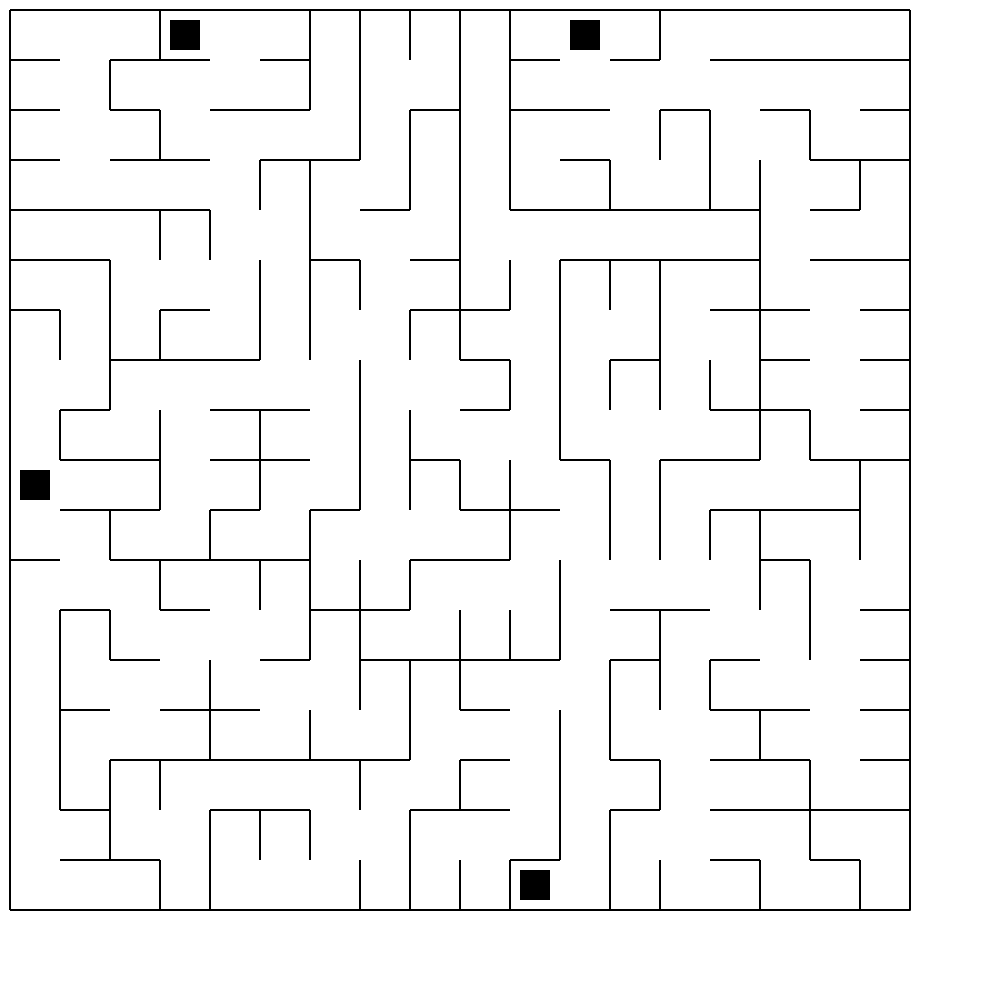
\includegraphics[scale=0.3]{img/canvas.png}
 \caption{Příklad bludiště vygenerovaného popsaným algoritmem s~falešnými cíli.}
 \label{fig:big}
\end{figure}

\newpage
~
\newpage

\section{Závěr}
Tato práce se zabývala algoritmy pro generování bludišť a jejich případnými aplikacemi. Byla objasněna souvislost
mezi generováním perfektních bludišť a kostrami grafu v~teorii grafů. V~práci byly popsány základní algoritmy
pro generování bludišť, vycházející z~grafových algoritmů pro hledání koster grafu. Byl popsán způsob využití
generování bludišť v~počítačových hrách, ve steganografii a možnosti generování třírozměrných bludišť.
Podrobněji byla také popsána metoda grafického generování, kdy se využívá černobílého rastrového
obrázku jako jisté šablony pro výsledné bludiště.

V~práci byla také popsána vlastní modifikace, která se zabývala generováním potenciálně řídkých bludišť s~falešnými cíli.
Tato modifikace je založena na rozdělení grafu do komponent souvislosti s~využitím myšlenky simulovaného žíhání 
a následné generování celého bludiště. Celý algoritmus byl implementován v~jazyce JavaScript.


\newpage
\enlargethispage*{2em}
\bibliographystyle{czplain}
\bibliography{literatura}{}
 
\end{document}